\documentclass[preprint, hmargin=1in, vmargin=1in]{aastex62}
%%%%%%begin preamble
%\usepackage[hmargin=1in, vmargin=1in]{geometry} % Margins
\usepackage{hyperref}
\usepackage{url}
\usepackage{natbib}
\setlength{\bibsep}{0pt plus 0.3ex}
\usepackage{graphicx}
\usepackage{amsmath}
\usepackage{amsfonts}
\usepackage{amssymb}
%\usepackage{import}
\usepackage{wrapfig}

\usepackage{color}
\hypersetup{
  colorlinks   = true,
  %citecolor    = blue
  citecolor    = gray
  % gray is not being found!?!
  % gray is found if pdfpages is used... crap.
  %citecolor    = grey
  %citecolor    = Gray
}

%% headers
\usepackage{fancyhdr}
\pagestyle{fancy}
\fancyhf{} % sets both header and footer to nothing
\lhead{Evan Anders -- Research Proposal}
\rhead{NASA Hubble Fellowship Program}
\cfoot{\footnotesize{\thepage}}
%\pagestyle{empty}
%\pagenumbering{gobble}
%\renewcommand*{\thefootnote}{\fnsymbol{footnote}}

\renewcommand{\vec}{\ensuremath{\boldsymbol}}
\newcommand{\dedalus}{\href{http://dedalus-project.org}{Dedalus}}
\newcommand{\del}{\ensuremath{\vec{\nabla}}}
\newcommand{\scrS}{\ensuremath{\mathcal{S}}}

\newcommand{\prf}{Physical Review Fluids}

%\newcommand{\nosection}[1]{%
%  \refstepcounter{section}%
%  \addcontentsline{toc}{section}{\protect\numberline{\thesection}#1}%
%  \markright{#1}}
%\newcommand{\nosubsection}[1]{%
%  \refstepcounter{subsection}%
%  \addcontentsline{toc}{subsection}{\protect\numberline{\thesubsection}#1}%
%  \markright{#1}}

%\usepackage{atbegshi}
%%%%%%end preamble


\begin{document}
\begin{center}
\Large{Convective Conundrums in the Asteroseismic Age:\\\vspace{-6pt}The interplay of rotation and magnetism in stellar convection} \\
\large{Evan H. Anders }
\end{center}
\vspace{-0.2cm}



Main sequence stars with masses similar to the Sun rely on vigorous near-surface convective regions to transport their stellar luminosity.
These convecting regions are highly stratified (14 density scale heights in the Sun), and the convective motions generate sound waves which refract due to stratification as they propagate into the stellar interior.
Helioseismology and asteroseismology measure the surface signatures of these acoustic waves---and gravity modes when available---to examine the interior of the Sun and other stars.
These measurements have enabled the precise determination of mass and radius of many stars, and have revealed the interior structure and mean flows, like differential rotation, inside the Sun \citep{huber&all2019, christensen-dalsgaard2002}.

Interpretation of asteroseismic and helioseismic data relies on one-dimensional (1D) stellar structure models. 
State-of-the-art codes like MESA \citep{paxton&all2011} which generate 1D stellar structure profiles have many deficiencies \citep{buldgen2019}, including their reliance on parameterizations of convection like mixing length theory \citep[MLT,][]{bohm-vitense1958}.
MLT assumes that convective flows with length scales proportional to the local density scale height are driven throughout the full depth of the convective zone.
This theory thus predicts that small convective elements driven near the stellar surface---like the ``granules'' we see on the Sun's surface---should exist on top of large-scale ``giant cells'' driven in the deep convection zone.
Unfortunately, modern helioseismic observations and direct measurements of flows on the Sun's surface have not detected giant cells \citep{hanasoge&all2015, hathaway&all2015}.
The absence of these flows has called into question our most fundamental understanding of the nature of convection in stars, a problem widely referred to as the ``Solar Convective Conundrum.''
Improving our understanding of convection, and thus improving stellar structure models is critical to improving asteroseismic observations.
With NASA's TESS mission currently underway and supplying more than $10^4$ asteroseismic target stars in its nominal mission, and with other missions such as WFIRST increasing the number of asteroseismic target stars to $10^6$ in the next decade \citep{huber&all2019}, we must sort out the convective conundrum.

My research aims to  help solve this Convective Conundrum by gaining a better understanding of convection in the highly stratified, rotating, magnetized context of stellar convection.
Parameterizations like MLT generally neglect stellar rotation and magnetism, but modern asteroseismic observations have detected latitudinal differential rotation in stars \citep{benomar&all2018} and shown that the structure of stellar magnetic fields affects asteroseismic measurements \citep{santos&all2018}.
As a Hubble fellow, I will conduct a series of studies which will span from the smallest to the largest scales present in stellar convection to better understand the importance of rotation and magnetism on stellar convection and structure.
I will build up understanding in detailed, small-scale studies to later inform the production and interpretation of large-scale global studies.

\vspace{-55pt}
\section*{\textbf{Numerical Explorations of the Entropy Rain Hypothesis}}
\paragraph{The Entropy Rain hypothesis}
In incompressible convection, velocity and temperature fields are symmetrical in upflows and downflows.
This symmetry is broken when convection occurs in the presence of atmospheric density stratification.
Stratified convection exhibits upwellings that are slow, weak, and wide in balance with downflows which are intense, fast, and narrow.
It has been hypothesized that downflows may be so powerful in the context of solar-like convection that they alone transport the stellar luminosity.
These downflows would exist alongside mass-conserving upflows which exhibit negligible energy transport.
This ``entropy rain'' hypothesis, first suggested by \citet{spruit1997}, is gaining traction, and could explain the absence of giant cells in observations \citep{hanasoge&all2015}.
Recent simulations of solar-like convection suggest that surface-driven downflows can indeed transport most of the stellar luminosity \citep{kapyla&all2017}, and recent theoretical work showed that such a concept could be included into 1D parameterizations \citep{brandenburg2016}.
A schematic of the entropy rain picture is shown in Fig.~\ref{fig:tri_panel}a.


\paragraph{Convection at the smallest scales: individual downflows} 
Regardless of the veracity of the entropy rain hypothesis, these modern studies suggest that the nonlocal effects of stellar downflows deserve more careful study.
It is possible these downflows turbulently break up into distinct pieces as they fall and these individual downflow pieces can be modeled as ``thermals.''
Thermals are regions of cold fluid which accelerate due to buoyancy forces and shape themselves into vortex rings; an evolved turbulent thermal is visualized in Fig. \ref{fig:tri_panel}b.
Thermals are also observed and studied in the Earth's atmosphere \citep{lecoanet&jeevanjee2019}.

\begin{figure*}[t]
    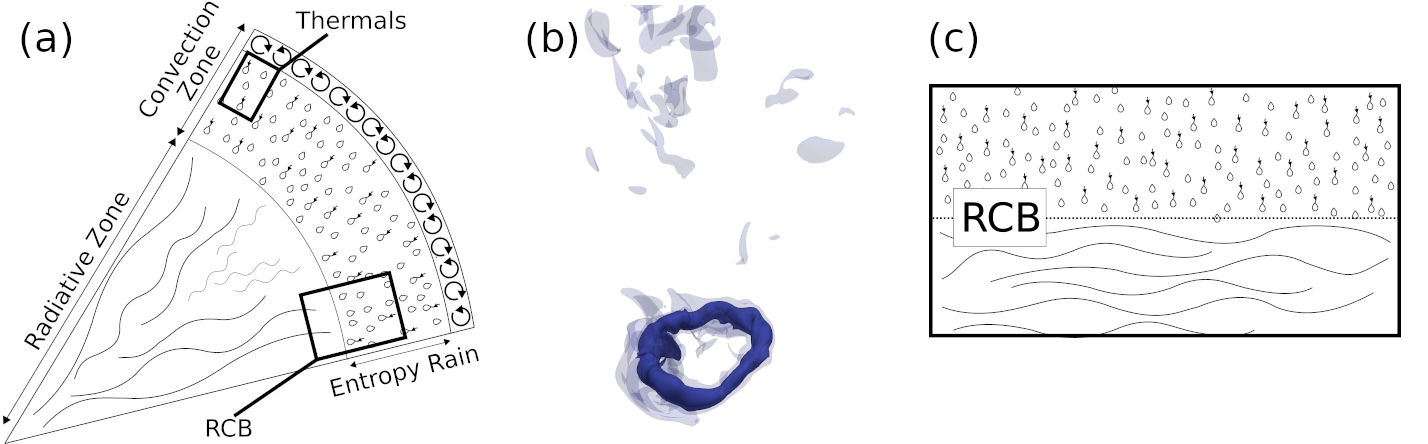
\includegraphics[width=\textwidth]{./figs/tri_panel.png}
    \caption{ (a) A schematic of the interior of solar-type stars under the entropy rain hypothesis, where cold droplets of fluid carry the stellar luminosity below a small traditional convective surface layer.
	The scope of the two experiments described in this section are boxed and labeled (``Thermals'' and ``RCB'').
	(b) A 3D visualization of entropy perturbations within the downward-propagating reference frame of a turbulent thermal, which may be the dynamical form of entropy rain.
	(c) A schematic of the radiative-convective boundary (RCB), where downflows impinge upon a stable layer and excite gravity waves within that layer.
	\label{fig:tri_panel} }
\end{figure*}


Throughout my PhD, I used the open-source Dedalus \citep{burns&all2019} code to study questions about stellar convection at various scales, and I recently used Dedalus to study thermals-as-downflows \citep{andersLB2019}.
I learned how atmospheric stratification affects the propagation of these downflows.
Surprisingly, I found that these downflows carry enough energy to feasibly transport the stellar luminosity, giving credence to the entropy rain hypothesis.
However, this work neglected turbulence, magnetism, and rotation, which are key ingredients in stellar convection.

As a Hubble fellow, I will build upon this study from my thesis work to understand if entropy rain is feasible by learning how rotation, magnetism, and turbulence affect the ability of these downflows to transit a stellar convection zone.
These physical complications could all have filtering effects on downflows, preventing their successful propagation through the stellar convection zone in certain regimes.
I will determine whether strong magnetic fields or rapid global rotation can ``evaporate'' entropy rain.
While \citet{lecoanet&jeevanjee2019} found that turbulence had little effect on the evolution of thermals in unstratified atmospheres, the compressional effects of atmospheric stratification could change this outcome, and I will explore this possibility.
Constraining the regimes in which these realistic effects prevent downflows from crossing the stellar convection zone is crucial to determining the validity of the entropy rain hypothesis.

\paragraph{Convection at the mesoscale: interactions at the radiative-convective boundary}
In solar-type stars, a radiative-convective boundary (RCB) sits at the base of the convection zone; at the RCB, turbulent convective motions give way to a stably stratified radiative zone where radiation effectively carries the stellar luminosity.
In the Sun, the RCB is characterized by a transition from moderate instability to strong stability.
The solar RCB furthermore coincides with a region of intense shear in the Sun's radial velocity profile called the tachocline, and it is thought that these shear interactions are a crucial driver of the Sun's magnetic dynamo.
Constraining the pumping of angular momentum and magnetism by downflows into the RCB is crucial to figuring out how the dynamos and differential rotation profiles of stars are driven.
Measurements suggest that the Sun's RCB is thin \citep{basu1997}, but many modern simulations produce RCBs which are up to an order of magnitude thicker than the solar one \citep{hotta2017}.
This suggests that many simulations are studying angular momentum and magnetic field pumping mechanisms in the wrong regime of ``stiffness'' of the RCB \citep{brummell&all2002, rogers&glatzmaier2005, couston&all2017}.

As a Hubble fellow, I will study how an ensemble of downflows interacts with a solar-like RCB in the presence of rotation and magnetism to learn how these interactions establish the stellar rotation profile and magnetic dynamo.
I will simulate time-evolving mesoscale convection where unstable convection zones overlay stable radiative interiors, as depicted in Fig.~\ref{fig:tri_panel}c.
This will naturally extends the work I performed in \citep{anders&brown2017, anders&all2019} in setups similar to those in \citep{kapyla&all2017} where downflows were found to be dominant. 
These simulations will be conducted in the regimes where my downflow-only thermals simulations predict that downflows are not filtered out by rotation and magnetism.
If downflows are capable of effectively pumping magnetism and angular momentum into the RCB, the popular picture of the RCB and tachocline as drivers of stellar dynamos will be validated.
If downflows cannot carry these quantities into the RCB, then magnetic fields are likely generated by another process.
In addition to helping determine where stellar dynamos are driven, these studies will help determine the stellar rotation rates and luminosities in which downflows can effectively establish solar-like differential rotation profiles through RCB interactions, building on the recent theoretical work of \citep{wood&brummell2018}.

\section*{\textbf{Global scale convection: dynamics in relaxed atmospheres}}
MLT's deficiencies have led researchers to seek out ways to couple 1D models with fully convective, three-dimensional (3D) global simulations in order to replace convective parameterizations with real sampled convective statistics.
Recently, 3D spherical shell simulations of convection in a thin, near-surface layer have been successfully coupled to 1D models by \citet{jorgensen&weiss2019}.
Unfortunately, the large computational expense of 3D simulations meant that this coupling could not occur at runtime but was instead performed \emph{a posteriori}.
Furthermore, near-surface simulations examine a regime where the convective overturn timescale is very similar to the local Kelvin-Helmoltz (KH) timescale of atmospheric equilibration.
In studies of deep convection, where most disagreements between simulations and observations occur \citep{hanasoge&all2015}, these timescales become disparate, and many overturn timescales pass during one KH timescale.
Simulations of deep convection must therefore either take measurements in a disequilibrium state or waste a vast amount of computational time waiting for the atmospheric structure and mean flows to become statistically stationary.

Equilibrated solutions are required for coupling with 1D models, and in order to enable 3D-to-1D coupling of deep convection for arbitrary stars, we must employ clever numerical techniques rather than traditional timestepping alone.
During my PhD, I created and verified an ``accelerated evolution'' tool which skips the long KH timescale in convective simulations \citep{anders&all2018}.
This tool accurately (results differed from traditional timestepping by less than 1\%) reached a relaxed, equilibrated state using an order of magnitude fewer computational resources than a simulation which timestepped through a full KH timescale.

\begin{wrapfigure}{r}{0.3\textwidth}
	\begin{center}
	\vspace{-10pt}
    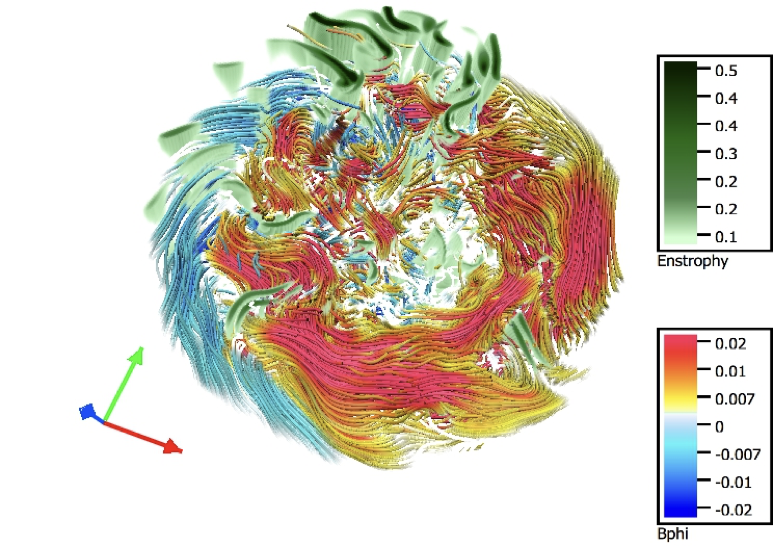
\includegraphics[width=0.28\textwidth]{./figs/mdwarf.png}
	\vspace{-16pt}
	\end{center}
    \caption{A volume rendering of a global dynamo simulation in Dedalus.
	Enstrophy, or the magnitude of vorticity, is shown in green.
	Red and blue lines denote the magnitude and direction of azimuthal magnetic field.
	\label{fig:mdwarf} }
\end{wrapfigure}


As a Hubble fellow, I will extend my accelerated evolution method by creating and validating a generalized public module which rapidly equilibrates mean thermodynamic profiles and flows in global simulations.
I will use Dedalus, which can accurately simulate deep convective motions in global domains which include the origin at $r = 0$ \citep[as visualized in Fig.~\ref{fig:mdwarf}, and tested in][]{lecoanet&all2019}, to test the accuracy of this tool.
%The large-scale structures seen in Fig.~\ref{fig:mdwarf} arise quickly, but the equilibration and saturation of these structures and other simulation measurements often takes KH timescales which cannot be feasibly simulated in turbulent regimes.
This module will read in statistical measures from unequilibrated convective simulations and output the properly equilibrated mean state.
Researchers simulating global convection using arbitrary codes will be able to use this module to rapidly equilibrate simulations with state-of-the-art turbulent dynamics.
Statistics of deep convection can be sampled from these converged states and coupled with 1D models in the same manner as \citet{jorgensen&weiss2019} coupled simulations of surface convection.
In my own research, I will employ this tool to study converged deep convection in the same dynamical regimes as my previous mesoscale studies to examine RCB interactions in a spherical geometry.
Furthermore, \citet{featherstone&hindman2016} found that rapid rotation could in some cases suppress giant cells in global simulations, and I will determine if this suppression of giant cells occurs in regimes where my individual downflow studies determined that entropy rain could cross the convection zone.


\section*{\textbf{Relevance to NASA Astrophysics \& Justification of Institute}}
Improving stellar structure \& evolution models is crucial to determining our cosmic origins and answering the question, ``How did we get here?''
Convective processes are important in all stars and influence determinations of stellar mass, radius, or age.
Asteroseismology can measure the masses and the radii of stars with exoplanets, and can constrain properties of large stellar populations for uses in galactic archaeology.
Uncertainties in our convective models, which the Convective Conundrum have made clear, limit the accuracy of these techniques, and in doing so impede studies of exoplanets and galactic archaeology by missions like TESS, JWST, and WFIRST.
To understand how we got here, we need to improve stellar structure models by learning more about convection.

Northwestern university, and specifically the Center for Interdisciplinary Exploration and Research in Astrophysics (CIERA), is the perfect location for me to carry out this proposed work.
Prof.~Daniel Lecoanet is a core developer of Dedalus and will be my primary advisor and collaborator at CIERA.
His past work on thermals \citep{lecoanet&jeevanjee2019, tarshish&all2018}, convection \citep{lecoanet&quataert2013, lecoanet&all2014}, convection-stable layer interactions \citep{lecoanet&all2016, couston&all2017}, rotating convection \citep{couston&all2019}, and global simulations \citep{lecoanet&all2019} will make him a valuable collaborator and advisor for the projects proposed here.
Furthermore, I have already published a paper on thermals in close collaboration with Prof.~Lecoanet \citep{andersLB2019}, which the work proposed here naturally extends.
I will also collaborate with Prof.~Yoram Lithwick, who has expertise on rotating convection \citep[e.g.,][]{BDLithwick2014}.
CIERA houses many experts in computational fluid dynamics beyond Profs.~Lecoanet \& Lithwick, such as Profs.~Sasha Tchekhovskoy \& Claude-Andre Faucher-Giguere.
I look forward to joining the astrophysical fluid dynamics group at CIERA where I will have many opportunities to discuss and develop new numerical techniques, strategies, and applications across astrophysics.


\bibliographystyle{yahapj}
\bibliography{biblio}
\end{document}
